% Generated by Sphinx.
\def\sphinxdocclass{report}
\documentclass[a4paper,12pt,ngerman]{sphinxmanual}
\usepackage[utf8]{inputenc}
\DeclareUnicodeCharacter{00A0}{\nobreakspace}
\usepackage{cmap}
\usepackage[T1]{fontenc}
\usepackage[ngerman]{babel}
\usepackage{times}
\usepackage[Sonny]{fncychap}
\usepackage{longtable}
\usepackage{sphinx}
\usepackage{multirow}
\usepackage{multicol}


\title{Meshkit Documentation}
\date{26. 10. 2013}
\release{0.0.2}
\author{Manuel Munz}
\newcommand{\sphinxlogo}{}
\renewcommand{\releasename}{Version}
\makeindex

\makeatletter
\def\PYG@reset{\let\PYG@it=\relax \let\PYG@bf=\relax%
    \let\PYG@ul=\relax \let\PYG@tc=\relax%
    \let\PYG@bc=\relax \let\PYG@ff=\relax}
\def\PYG@tok#1{\csname PYG@tok@#1\endcsname}
\def\PYG@toks#1+{\ifx\relax#1\empty\else%
    \PYG@tok{#1}\expandafter\PYG@toks\fi}
\def\PYG@do#1{\PYG@bc{\PYG@tc{\PYG@ul{%
    \PYG@it{\PYG@bf{\PYG@ff{#1}}}}}}}
\def\PYG#1#2{\PYG@reset\PYG@toks#1+\relax+\PYG@do{#2}}

\expandafter\def\csname PYG@tok@gd\endcsname{\def\PYG@tc##1{\textcolor[rgb]{0.63,0.00,0.00}{##1}}}
\expandafter\def\csname PYG@tok@gu\endcsname{\let\PYG@bf=\textbf\def\PYG@tc##1{\textcolor[rgb]{0.50,0.00,0.50}{##1}}}
\expandafter\def\csname PYG@tok@gt\endcsname{\def\PYG@tc##1{\textcolor[rgb]{0.00,0.27,0.87}{##1}}}
\expandafter\def\csname PYG@tok@gs\endcsname{\let\PYG@bf=\textbf}
\expandafter\def\csname PYG@tok@gr\endcsname{\def\PYG@tc##1{\textcolor[rgb]{1.00,0.00,0.00}{##1}}}
\expandafter\def\csname PYG@tok@cm\endcsname{\let\PYG@it=\textit\def\PYG@tc##1{\textcolor[rgb]{0.25,0.50,0.56}{##1}}}
\expandafter\def\csname PYG@tok@vg\endcsname{\def\PYG@tc##1{\textcolor[rgb]{0.73,0.38,0.84}{##1}}}
\expandafter\def\csname PYG@tok@m\endcsname{\def\PYG@tc##1{\textcolor[rgb]{0.13,0.50,0.31}{##1}}}
\expandafter\def\csname PYG@tok@mh\endcsname{\def\PYG@tc##1{\textcolor[rgb]{0.13,0.50,0.31}{##1}}}
\expandafter\def\csname PYG@tok@cs\endcsname{\def\PYG@tc##1{\textcolor[rgb]{0.25,0.50,0.56}{##1}}\def\PYG@bc##1{\setlength{\fboxsep}{0pt}\colorbox[rgb]{1.00,0.94,0.94}{\strut ##1}}}
\expandafter\def\csname PYG@tok@ge\endcsname{\let\PYG@it=\textit}
\expandafter\def\csname PYG@tok@vc\endcsname{\def\PYG@tc##1{\textcolor[rgb]{0.73,0.38,0.84}{##1}}}
\expandafter\def\csname PYG@tok@il\endcsname{\def\PYG@tc##1{\textcolor[rgb]{0.13,0.50,0.31}{##1}}}
\expandafter\def\csname PYG@tok@go\endcsname{\def\PYG@tc##1{\textcolor[rgb]{0.20,0.20,0.20}{##1}}}
\expandafter\def\csname PYG@tok@cp\endcsname{\def\PYG@tc##1{\textcolor[rgb]{0.00,0.44,0.13}{##1}}}
\expandafter\def\csname PYG@tok@gi\endcsname{\def\PYG@tc##1{\textcolor[rgb]{0.00,0.63,0.00}{##1}}}
\expandafter\def\csname PYG@tok@gh\endcsname{\let\PYG@bf=\textbf\def\PYG@tc##1{\textcolor[rgb]{0.00,0.00,0.50}{##1}}}
\expandafter\def\csname PYG@tok@ni\endcsname{\let\PYG@bf=\textbf\def\PYG@tc##1{\textcolor[rgb]{0.84,0.33,0.22}{##1}}}
\expandafter\def\csname PYG@tok@nl\endcsname{\let\PYG@bf=\textbf\def\PYG@tc##1{\textcolor[rgb]{0.00,0.13,0.44}{##1}}}
\expandafter\def\csname PYG@tok@nn\endcsname{\let\PYG@bf=\textbf\def\PYG@tc##1{\textcolor[rgb]{0.05,0.52,0.71}{##1}}}
\expandafter\def\csname PYG@tok@no\endcsname{\def\PYG@tc##1{\textcolor[rgb]{0.38,0.68,0.84}{##1}}}
\expandafter\def\csname PYG@tok@na\endcsname{\def\PYG@tc##1{\textcolor[rgb]{0.25,0.44,0.63}{##1}}}
\expandafter\def\csname PYG@tok@nb\endcsname{\def\PYG@tc##1{\textcolor[rgb]{0.00,0.44,0.13}{##1}}}
\expandafter\def\csname PYG@tok@nc\endcsname{\let\PYG@bf=\textbf\def\PYG@tc##1{\textcolor[rgb]{0.05,0.52,0.71}{##1}}}
\expandafter\def\csname PYG@tok@nd\endcsname{\let\PYG@bf=\textbf\def\PYG@tc##1{\textcolor[rgb]{0.33,0.33,0.33}{##1}}}
\expandafter\def\csname PYG@tok@ne\endcsname{\def\PYG@tc##1{\textcolor[rgb]{0.00,0.44,0.13}{##1}}}
\expandafter\def\csname PYG@tok@nf\endcsname{\def\PYG@tc##1{\textcolor[rgb]{0.02,0.16,0.49}{##1}}}
\expandafter\def\csname PYG@tok@si\endcsname{\let\PYG@it=\textit\def\PYG@tc##1{\textcolor[rgb]{0.44,0.63,0.82}{##1}}}
\expandafter\def\csname PYG@tok@s2\endcsname{\def\PYG@tc##1{\textcolor[rgb]{0.25,0.44,0.63}{##1}}}
\expandafter\def\csname PYG@tok@vi\endcsname{\def\PYG@tc##1{\textcolor[rgb]{0.73,0.38,0.84}{##1}}}
\expandafter\def\csname PYG@tok@nt\endcsname{\let\PYG@bf=\textbf\def\PYG@tc##1{\textcolor[rgb]{0.02,0.16,0.45}{##1}}}
\expandafter\def\csname PYG@tok@nv\endcsname{\def\PYG@tc##1{\textcolor[rgb]{0.73,0.38,0.84}{##1}}}
\expandafter\def\csname PYG@tok@s1\endcsname{\def\PYG@tc##1{\textcolor[rgb]{0.25,0.44,0.63}{##1}}}
\expandafter\def\csname PYG@tok@gp\endcsname{\let\PYG@bf=\textbf\def\PYG@tc##1{\textcolor[rgb]{0.78,0.36,0.04}{##1}}}
\expandafter\def\csname PYG@tok@sh\endcsname{\def\PYG@tc##1{\textcolor[rgb]{0.25,0.44,0.63}{##1}}}
\expandafter\def\csname PYG@tok@ow\endcsname{\let\PYG@bf=\textbf\def\PYG@tc##1{\textcolor[rgb]{0.00,0.44,0.13}{##1}}}
\expandafter\def\csname PYG@tok@sx\endcsname{\def\PYG@tc##1{\textcolor[rgb]{0.78,0.36,0.04}{##1}}}
\expandafter\def\csname PYG@tok@bp\endcsname{\def\PYG@tc##1{\textcolor[rgb]{0.00,0.44,0.13}{##1}}}
\expandafter\def\csname PYG@tok@c1\endcsname{\let\PYG@it=\textit\def\PYG@tc##1{\textcolor[rgb]{0.25,0.50,0.56}{##1}}}
\expandafter\def\csname PYG@tok@kc\endcsname{\let\PYG@bf=\textbf\def\PYG@tc##1{\textcolor[rgb]{0.00,0.44,0.13}{##1}}}
\expandafter\def\csname PYG@tok@c\endcsname{\let\PYG@it=\textit\def\PYG@tc##1{\textcolor[rgb]{0.25,0.50,0.56}{##1}}}
\expandafter\def\csname PYG@tok@mf\endcsname{\def\PYG@tc##1{\textcolor[rgb]{0.13,0.50,0.31}{##1}}}
\expandafter\def\csname PYG@tok@err\endcsname{\def\PYG@bc##1{\setlength{\fboxsep}{0pt}\fcolorbox[rgb]{1.00,0.00,0.00}{1,1,1}{\strut ##1}}}
\expandafter\def\csname PYG@tok@kd\endcsname{\let\PYG@bf=\textbf\def\PYG@tc##1{\textcolor[rgb]{0.00,0.44,0.13}{##1}}}
\expandafter\def\csname PYG@tok@ss\endcsname{\def\PYG@tc##1{\textcolor[rgb]{0.32,0.47,0.09}{##1}}}
\expandafter\def\csname PYG@tok@sr\endcsname{\def\PYG@tc##1{\textcolor[rgb]{0.14,0.33,0.53}{##1}}}
\expandafter\def\csname PYG@tok@mo\endcsname{\def\PYG@tc##1{\textcolor[rgb]{0.13,0.50,0.31}{##1}}}
\expandafter\def\csname PYG@tok@mi\endcsname{\def\PYG@tc##1{\textcolor[rgb]{0.13,0.50,0.31}{##1}}}
\expandafter\def\csname PYG@tok@kn\endcsname{\let\PYG@bf=\textbf\def\PYG@tc##1{\textcolor[rgb]{0.00,0.44,0.13}{##1}}}
\expandafter\def\csname PYG@tok@o\endcsname{\def\PYG@tc##1{\textcolor[rgb]{0.40,0.40,0.40}{##1}}}
\expandafter\def\csname PYG@tok@kr\endcsname{\let\PYG@bf=\textbf\def\PYG@tc##1{\textcolor[rgb]{0.00,0.44,0.13}{##1}}}
\expandafter\def\csname PYG@tok@s\endcsname{\def\PYG@tc##1{\textcolor[rgb]{0.25,0.44,0.63}{##1}}}
\expandafter\def\csname PYG@tok@kp\endcsname{\def\PYG@tc##1{\textcolor[rgb]{0.00,0.44,0.13}{##1}}}
\expandafter\def\csname PYG@tok@w\endcsname{\def\PYG@tc##1{\textcolor[rgb]{0.73,0.73,0.73}{##1}}}
\expandafter\def\csname PYG@tok@kt\endcsname{\def\PYG@tc##1{\textcolor[rgb]{0.56,0.13,0.00}{##1}}}
\expandafter\def\csname PYG@tok@sc\endcsname{\def\PYG@tc##1{\textcolor[rgb]{0.25,0.44,0.63}{##1}}}
\expandafter\def\csname PYG@tok@sb\endcsname{\def\PYG@tc##1{\textcolor[rgb]{0.25,0.44,0.63}{##1}}}
\expandafter\def\csname PYG@tok@k\endcsname{\let\PYG@bf=\textbf\def\PYG@tc##1{\textcolor[rgb]{0.00,0.44,0.13}{##1}}}
\expandafter\def\csname PYG@tok@se\endcsname{\let\PYG@bf=\textbf\def\PYG@tc##1{\textcolor[rgb]{0.25,0.44,0.63}{##1}}}
\expandafter\def\csname PYG@tok@sd\endcsname{\let\PYG@it=\textit\def\PYG@tc##1{\textcolor[rgb]{0.25,0.44,0.63}{##1}}}

\def\PYGZbs{\char`\\}
\def\PYGZus{\char`\_}
\def\PYGZob{\char`\{}
\def\PYGZcb{\char`\}}
\def\PYGZca{\char`\^}
\def\PYGZam{\char`\&}
\def\PYGZlt{\char`\<}
\def\PYGZgt{\char`\>}
\def\PYGZsh{\char`\#}
\def\PYGZpc{\char`\%}
\def\PYGZdl{\char`\$}
\def\PYGZhy{\char`\-}
\def\PYGZsq{\char`\'}
\def\PYGZdq{\char`\"}
\def\PYGZti{\char`\~}
% for compatibility with earlier versions
\def\PYGZat{@}
\def\PYGZlb{[}
\def\PYGZrb{]}
\makeatother

\begin{document}
\shorthandoff{"}
\maketitle
\tableofcontents
\phantomsection\label{index::doc}



\chapter{Allgemeine Infos zur Meshkit Freifunk Firmware}
\label{about:dokumentation-zu-meshkit}\label{about::doc}\label{about:allgemeine-infos-zur-meshkit-freifunk-firmware}\label{about:id1}

\section{Was ist Meshkit?}
\label{about:was-ist-meshkit}
Meshkit ist ein Generator für individualisierte Freifunk-Firmware-Images.


\section{Features}
\label{about:features}\begin{itemize}
\item {} 
Support für Communityprofile (verschiedene Einstellungen für unterschiedliche Communities

\item {} 
Erstellen vorkonfigurierter Firmwareimages, die direkt nach dem Flashen im Mesh erreichbar sind.

\item {} 
Pakete können direkt mit ins Image gebaut werden (spart Platz)

\item {} 
Eigene Dateien können mit ins Image gebaut werden

\end{itemize}


\chapter{Einbinden des Freifunkrouters ins eigene Netzwerk}
\label{get/integration-into-networks:einbinden-des-freifunkrouters-ins-eigene-netzwerk}\label{get/integration-into-networks::doc}

\section{LAN-Setup}
\label{get/integration-into-networks:lan-setup}
Der Router ist mit seinem WAN-Port üer einen Switch Teil des lokalen
Netzwerks. Eigene PCs sind ebenfalls mit diesem Switch verbunden.


\section{WAN-Setup}
\label{get/integration-into-networks:wan-setup}
Der Router ist mit seinem WAN-Port am Internet (z.B. Modem) angeschlossen.
Eigene PCs werden an den LAN-Ports des Routers angeschlossen oder verbinden
sich per WLAN.


\chapter{Firmware mit Meshkit generieren lassen}
\label{generate:sphinx}\label{generate:firmware-mit-meshkit-generieren-lassen}\label{generate::doc}

\section{Wichtige Infos zum Router sammeln}
\label{generate:infos-zum-router-sammeln}\label{generate:wichtige-infos-zum-router-sammeln}
Um eine passende Firmware für das eigene Routermodell zu generieren muss man
zunächst einige Daten zum Router kennen:
\begin{itemize}
\item {} 
Chipsatz

\item {} 
Chipsatz des/der WLAN-Interfaces

\item {} 
Größe des RAM

\item {} 
Größe des Flash-Speichers

\end{itemize}

Diese Daten finden man in der \href{http://wiki.openwrt.org/toh/start}{Table of Hardware} im OpenWrt Wiki. Zu den
meisten Routermodellen gibt es auch eine Detailseite mit weiteren Infos. Diese
Seite sollte man ebenfalls zumindest kurz überfliegen. Hier finden sich
im Allgemeinen auch Infos zum Flashen und zur Rettung des Routers falls beim
Flashen etwas so richtig schief ging.

Beispiel:

Wir wollen die Daten für einen TP-Link WR1043ND zusammentragen. In der
\href{http://wiki.openwrt.org/toh/start}{Table of Hardware} sehen wir folgendes:

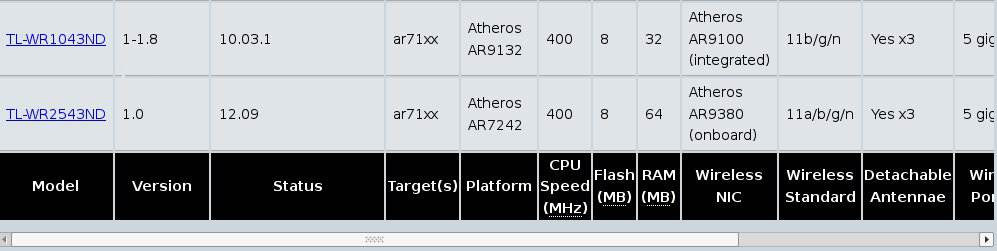
\includegraphics{toh-wr1043nd.jpg}

Daraus können wir entnehmen:
\begin{itemize}
\item {} 
Der Chipsatz gehört zur AR71XX Familie

\item {} 
WLAN benutzt Atheros Hardware

\item {} 
Der RAM ist 32 MB groß

\item {} 
Flash ist 8 MB groß

\end{itemize}


\section{IP-Adresse(n) registrieren}
\label{generate:ip-adresse-n-registrieren}
Nun muss noch mindestens eine IP-Adresse aus dem Freifunknetz für den Router
registriert werden. Hier hat jede Community ihre eigenen Seiten zur Registrierung,
im Allgemeinen kann man sich hier jedoch selbst bedienen und einfach eine noch
nicht vergebene Adresse für seinen Knoten reservieren.

Registrierungsseiten in den einzelnen Communities:
\begin{itemize}
\item {} 
\textbf{Augsburg:} Als Benutzer auf \href{http://augsburg.freifunk.net}{http://augsburg.freifunk.net} einloggen und ``Node registrieren''

\end{itemize}


\section{Firmware generieren}
\label{generate:firmware-generieren}
Das Erstellen von Firmwareimages erfolgt in drei Schritten:


\subsection{Grundlegende Systemeinstellungen}
\label{generate:grundlegende-systemeinstellungen}
Öffne die \href{http://meshkit.freifunk.net}{Meshkit} Webseite im Browser. Du siehst nun folgendes:

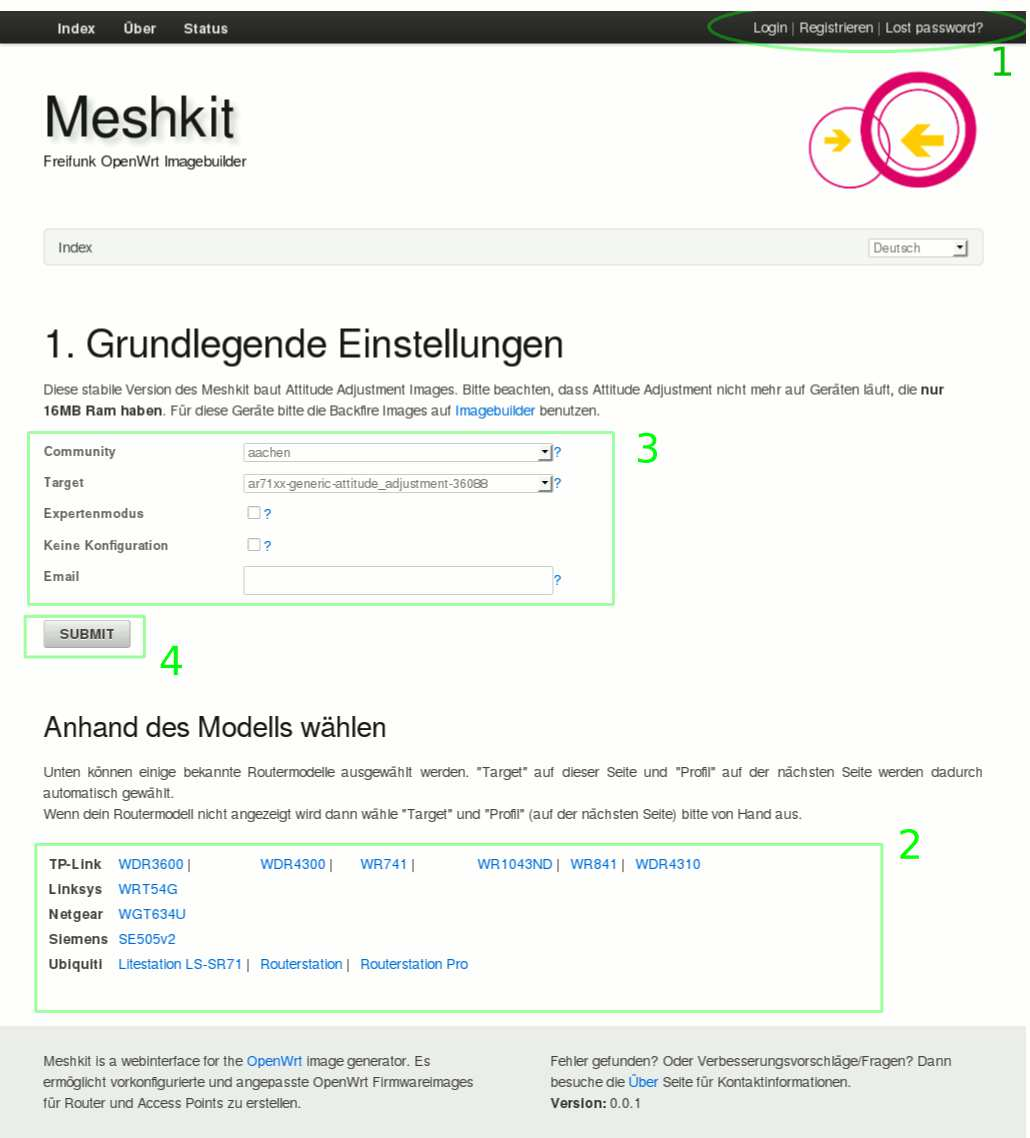
\includegraphics{basic-settings.jpg}

\emph{Erklärung:}
\begin{enumerate}
\item {} 
Login bzw. Registrieren
\begin{quote}

Hier kann man einen User für Meshkit registrieren. Dadurch wird es möglich,
einige Datenfelder beim Generieren neuer Images bereits auszufüllen, z.B.
Community, Adresse oder SSH Public Keys. Es ist nicht notwendig einen Benutzer
im Meshkit zu registrieren. Wer aber öfter Images generiert dem kann
die Registrierung ersparen, bei einigen Feldern immer und immer wieder die
selben Daten einzugeben.
\end{quote}

\item {} 
Geräte Vorauswahl
\begin{quote}

Im unteren Bereich von Meshkit befinden sich einige Links zu Geräten, die
häufig verwendet werden. Klickt man auf einen dieser links, dann wählt Meshkit
automatisch das richtige Target (und in Schritt 2 auch das passende Profil) für
dieses Gerät. Wenn ein Gerät nicht in dieser Liste steht dann heisst das nicht,
dass es nicht unterstützt wird, sondern nur, dass man Target und im nächsten
Schritt Profil manuell auswählen muss.
\end{quote}

\item {} 
Einstellungen
\begin{quote}

\begin{center}\begin{tabulary}{\linewidth}{|L|L|}
\hline
\textbf{\relax 
Option
} & \textbf{\relax 
Beschreibung
}\\\hline

Community
 & 
Wähle deine Community aus. (TODO: Was tun wenn es noch keine gibt?)
\\\hline

Target
 & 
Wähle ein passendes Target (siehe {\hyperref[generate:infos-zum-router-sammeln]{Infos zum Router sammeln}})
\\\hline

Expertenmodus
 & 
Wenn ausgewählt, dann werden im nächsten Schritt wesentlich mehr Optionen
zur Konfiguration des Routers angezeigt.
\\\hline

Keine Konfiguration
 & 
Erstellt ein Image, es wird aber keine Konfiguration durchgeführt. Dies
ist vor allem nützlich um Images zu erhalten, die für sysupgrade (TODO:
Seite zu sysupgrade anlegen) verwendet werden können.
\\\hline

Email
 & 
Wenn angegeben wird nachdem das Image gebaut wurde eine Mail an diese
Adresse geschickt.
\\\hline
\end{tabulary}\end{center}

\end{quote}

\item {} 
Absenden
\begin{quote}

Nachdem alle Einstellungen getätigt wurde klicke auf \textbf{Absenden} um zu
Schritt 2 des Meshkits zu gelangen, wo weitere Einstellungen vorgenommen
werden müssen.
\end{quote}

\end{enumerate}


\chapter{Erster Login}
\label{firstlogin::doc}\label{firstlogin:erster-login}
Nach dem Flashen des Routers sollte man sich entweder per Webinterface oder
per \code{ssh} mit dem Node verbinden, um das Passwort zu ändern.


\chapter{Benutzerhandbuch}
\label{usage/index::doc}\label{usage/index:benutzerhandbuch}

\section{Mit dem Router verbinden}
\label{usage/connect-router::doc}\label{usage/connect-router:mit-dem-router-verbinden}

\subsection{Netzwerkverbindung herstellen}
\label{usage/connect-router:netzwerkverbindung-herstellen}
Benötigt: Integrationsszenarien

Es gibt zwei Wege sich mit dem Router zu verbinden, um Status abzufragen
oder die Konfiguration zu ändern. Entweder man öffnet in
einem Browser die Webseite des Routers oder verbindet sich per ssh.


\section{Passwort ändern}
\label{usage/change-password::doc}\label{usage/change-password:passwort-andern}
Setzt voraus: Mit dem Router verbinden


\subsection{Im Webinterface}
\label{usage/change-password:im-webinterface}
Das Passwort kann unter \code{Administration -\textgreater{} System -\textgreater{} Administrator} geändert
werden.


\subsection{Mit SSH}
\label{usage/change-password:mit-ssh}
\begin{Verbatim}[commandchars=\\\{\}]
passwd
\end{Verbatim}

und zwei mal ein neues Passwort eingeben.


\chapter{Fortgeschrittene Konfiguration}
\label{advanced::doc}\label{advanced:fortgeschrittene-konfiguration}
Da die Meshkit Firmware auf dem vielseitigen OpenWrt basiert, gibt es viele
Möglichkeiten die Software auf dem Router für verschiedenste Einsatzzwecke
anzupassen.


\section{Eigene Dienste anbieten}
\label{advanced/offer-services::doc}\label{advanced/offer-services:eigene-dienste-anbieten}
Es ist möglich, im Freifunknetz eigene Dienste zur Verfügung zu stellen.


\subsection{Eigene Webseiten}
\label{advanced/websites:eigene-webseiten}\label{advanced/websites::doc}

\subsubsection{Lokal auf dem Node}
\label{advanced/websites:lokal-auf-dem-node}
Auf dem Freifunkrouter läuft ohnehin schon ein kleiner Webserver (\code{uhttpd}),
der verwendet werden kann um neben dem LuCI Webinterface auch eigene Inhalte per
HTTP zugänglich zu machen.


\paragraph{Seiten direkt über uhttpd ausliefern}
\label{advanced/websites:seiten-direkt-uber-uhttpd-ausliefern}
Es gibt die Möglichkeit direkt auf dem Node kleinere Seiten abzulegen, indem man
sie im Ordner /www unterbringt. Dies erfordert keine Änderung an der
Konfiguration des Nodes.
\paragraph{Einfache statische Seite}

\emph{Beispiel:}

\begin{Verbatim}[commandchars=\\\{\}]
\PYG{n+nt}{\PYGZlt{}html}\PYG{n+nt}{\PYGZgt{}}
  \PYG{n+nt}{\PYGZlt{}body}\PYG{n+nt}{\PYGZgt{}}
    Hallo Welt!
  \PYG{n+nt}{\PYGZlt{}/body\PYGZgt{}}
\PYG{n+nt}{\PYGZlt{}/html\PYGZgt{}}
\end{Verbatim}

Den obigen Code als \code{/www/hallowelt.html} abspeichern und danach im Browser
unter der Adresse \code{http://\textless{}nodeip\textgreater{}/hallowelt.html} aufrufen.
\paragraph{CGI-Scripte}

Möchte man CGI-Scripte ausführen, dann muss man diese in \code{/www/cgi-bin}
ablegen und ausführbar machen.

\emph{Beispiel:}

\begin{Verbatim}[commandchars=\\\{\}]
\PYG{c}{\PYGZsh{}!/bin/sh}

\PYG{n+nb}{echo} \PYG{l+s+s2}{\PYGZdq{}Content\PYGZhy{}type: text/html\PYGZdq{}}
\PYG{n+nb}{echo} \PYG{l+s+s2}{\PYGZdq{}\PYGZdq{}}

\PYG{n+nb}{echo} \PYG{l+s+s1}{\PYGZsq{}}
\PYG{l+s+s1}{\PYGZlt{}html\PYGZgt{}}
\PYG{l+s+s1}{  \PYGZlt{}head\PYGZgt{}}
\PYG{l+s+s1}{    \PYGZlt{}meta http\PYGZhy{}equiv=\PYGZdq{}Content\PYGZhy{}Type\PYGZdq{} content=\PYGZdq{}text/html; charset=UTF\PYGZhy{}8\PYGZdq{}\PYGZgt{}}
\PYG{l+s+s1}{    \PYGZlt{}title\PYGZgt{}Hallo Welt\PYGZlt{}/title\PYGZgt{}}
\PYG{l+s+s1}{  \PYGZlt{}/head\PYGZgt{}}
\PYG{l+s+s1}{  \PYGZlt{}body\PYGZgt{}}
\PYG{l+s+s1}{    Hallo Welt!}
\PYG{l+s+s1}{  \PYGZlt{}/body\PYGZgt{}}
\PYG{l+s+s1}{\PYGZlt{}/html\PYGZgt{}}
\PYG{l+s+s1}{\PYGZsq{}}
\end{Verbatim}

Den obigen Code als \code{/www/cgi-bin/helloworld.cgi} speichern und ausführbar
machen mit:

\begin{Verbatim}[commandchars=\\\{\}]
chmod +x /www/cgi\PYGZhy{}bin/helloworld.cgi
\end{Verbatim}

Dieses Testscript kann nun im Browser unter
\code{http://\textless{}nodeip\textgreater{}/cgi-bin/helloworld.cgi} abgerufen werden.

Das selbe Script in Lua:

\begin{Verbatim}[commandchars=\\\{\}]
\PYG{c+cp}{\PYGZsh{}!/usr/bin/lua}

\PYG{n+nb}{print}\PYG{p}{(}\PYG{l+s+s2}{\PYGZdq{}}\PYG{l+s}{C}\PYG{l+s}{o}\PYG{l+s}{n}\PYG{l+s}{t}\PYG{l+s}{e}\PYG{l+s}{n}\PYG{l+s}{t}\PYG{l+s}{\PYGZhy{}}\PYG{l+s}{t}\PYG{l+s}{y}\PYG{l+s}{p}\PYG{l+s}{e}\PYG{l+s}{:}\PYG{l+s}{ }\PYG{l+s}{t}\PYG{l+s}{e}\PYG{l+s}{x}\PYG{l+s}{t}\PYG{l+s}{/}\PYG{l+s}{h}\PYG{l+s}{t}\PYG{l+s}{m}\PYG{l+s}{l}\PYG{l+s}{\PYGZdq{}}\PYG{p}{)}
\PYG{n+nb}{print}\PYG{p}{(}\PYG{l+s+s2}{\PYGZdq{}}\PYG{l+s}{\PYGZdq{}}\PYG{p}{)}

\PYG{n+nb}{print} \PYG{p}{(}\PYG{l+s}{[[}
\PYG{l+s}{\PYGZlt{}html\PYGZgt{}}
\PYG{l+s}{  \PYGZlt{}head\PYGZgt{}}
\PYG{l+s}{    \PYGZlt{}meta http\PYGZhy{}equiv=\PYGZdq{}Content\PYGZhy{}Type\PYGZdq{} content=\PYGZdq{}text/html; charset=UTF\PYGZhy{}8\PYGZdq{}\PYGZgt{}}
\PYG{l+s}{    \PYGZlt{}title\PYGZgt{}Hello World\PYGZlt{}/title\PYGZgt{}}
\PYG{l+s}{  \PYGZlt{}/head\PYGZgt{}}
\PYG{l+s}{  \PYGZlt{}body\PYGZgt{}}
\PYG{l+s}{    Hallo Welt!}
\PYG{l+s}{  \PYGZlt{}/body\PYGZgt{}}
\PYG{l+s}{\PYGZlt{}/html\PYGZgt{}}
\PYG{l+s}{]]}\PYG{p}{)}
\end{Verbatim}


\paragraph{Verzeichnisinhalte}
\label{advanced/websites:verzeichnisinhalte}
In der Standardkonfiguration zeigt uhttpd auch Verzeichnisinhalte von
Verzeichnissen an, die keine index-Datei enthalten.

\emph{Beispiel:}

\begin{Verbatim}[commandchars=\\\{\}]
mkdir /www/verzeichnis
\PYG{n+nb}{echo} \PYG{l+s+s2}{\PYGZdq{}hallo\PYGZdq{}} \PYGZgt{} /www/verzeichnis/hallo.txt
\end{Verbatim}

Öffnet man im Browser jetzt \href{http:/}{http:/}/\textless{}nodeip\textgreater{}/verzeichnis, dann erhält man
folgende Ausgabe:

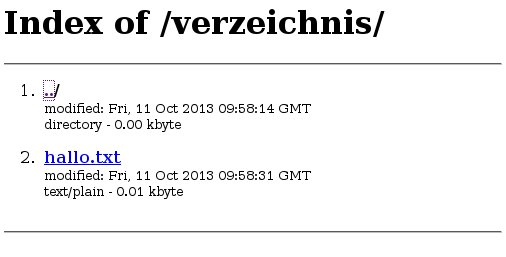
\includegraphics{directory-listing.jpg}


\subsubsection{Auf einem seperaten PC/Server}
\label{advanced/websites:auf-einem-seperaten-pc-server}
Soll die Webseite von einem anderen PC bzw. Server ausgeliefert werden,
der per Netzwerk mit dem Node verbunden ist gibt es mehrere Möglichkeiten,
diese Inhalte im Freifunknetz verfügbar zu machen.


\paragraph{Portforwarding}
\label{advanced/websites:portforwarding}
Auf dem Node wird ein Portforwarding eingerichtet, das einkommende Pakete
an den Webserver im eigenen Netzwerk weiterleitet. Siehe: Portforwarding (TODO)


\paragraph{HNA}
\label{advanced/websites:hna}
Mit HNA (Host Network Announcement) kann auf dem Node ein verfügbarer
IP-Bereich oder auch nur eine einzelne Adresse im Netzwerk bekannt gemacht
werden. So ist der Webserver direkt im Mesh erreichbar, muss jedoch selbst
nich OLSR nutzen. Siehe HNA für Rechner im eigenen Netz (TODO)


\paragraph{Server direkt ins OLSR Netz}
\label{advanced/websites:server-direkt-ins-olsr-netz}
Indem der Server selbst OLSR ``spricht'' kann er direkt aus dem Mesh erreichbar
sein. Siehe: OLSR im eigenen Netz (TODO)


\subsection{Dienste ankündigen mit dem Nameservice Plugin}
\label{advanced/nameservice::doc}\label{advanced/nameservice:dienste-ankundigen-mit-dem-nameservice-plugin}
Um eigene Dienste im gesamten Mesh bekannt zu machen kann das OLSR-Nameservice
Plugin verwendet werden. Dieses sendet in regelmässigen Abständen Informationen
über die lokalen Dienste an alle anderen Nodes im Mesh.

Es können nur Service-Ankündigungen für IPs/Adressen verschickt werden, die
entweder local verwendet oder als HNA angekündigt werden.

Ist der Service unter einer DNS-Adresse bekannt, dann kann statt einer IP auch
diese Adresse in der URL des Dienstes verwendet werden.


\subsubsection{Einrichtung}
\label{advanced/nameservice:einrichtung}
Ziel: Es soll ein Webserver auf dem lokalen Knoten mit der IP
10.11.12.13 angekündigt werden. Der Webserver läuft auf Port 80.


\paragraph{Einrichtung über LuCI}
\label{advanced/nameservice:einrichtung-uber-luci}
1. Um zu den Einstellungen für das Nameservice Plugin zu kommen: Gehe zu \emph{Dienste -\textgreater{} OLSR -\textgreater{} Plugins}
\begin{quote}

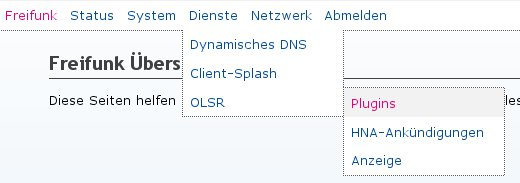
\includegraphics{nameservice-menu.jpg}
\end{quote}

2. Klicke in der Zeile wo olsrd\_nameservice.so.0.3 steht auf ``Bearbeiten''
\begin{quote}

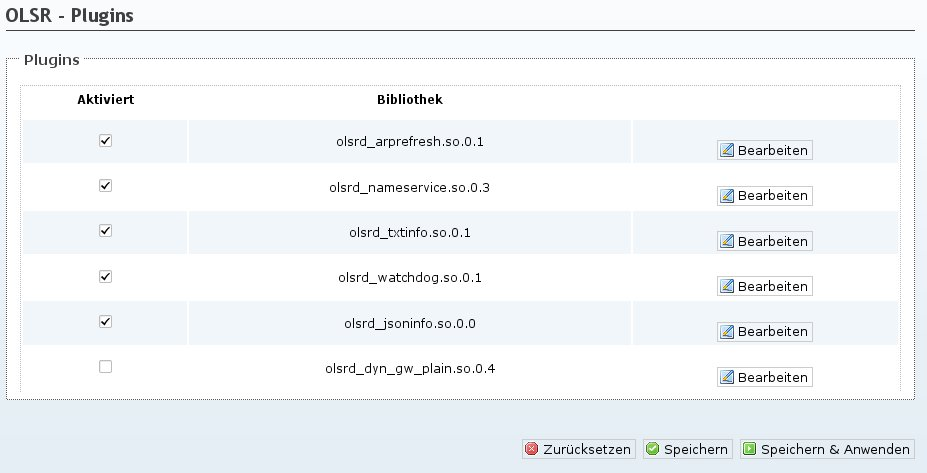
\includegraphics{nameservice-olsr-plugins.jpg}
\end{quote}

3. Füge unten aus der Auswahlbox eine Option für ``Service'' hinzu
\begin{quote}

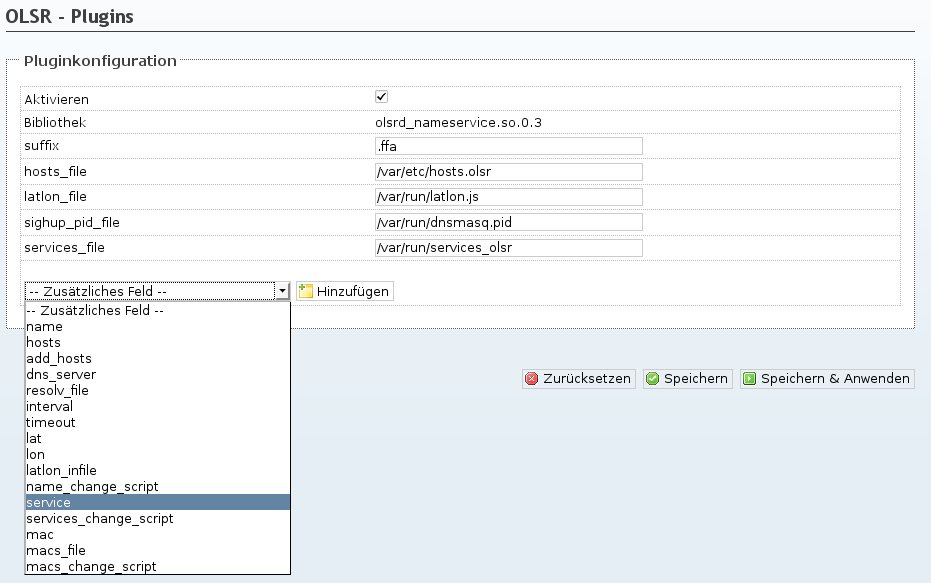
\includegraphics{nameservice_add_service.jpg}
\end{quote}

4. Plugin konfigurieren
\begin{quote}

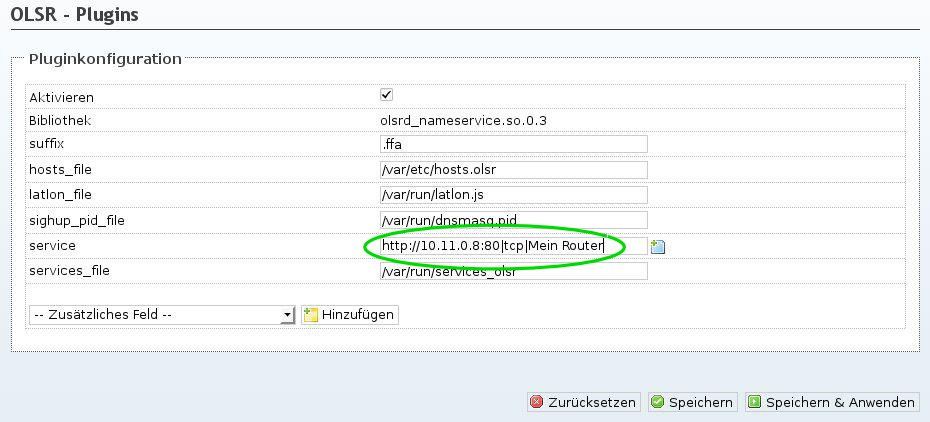
\includegraphics{Nameservice-einstellungen-service.jpg}
\end{quote}


\paragraph{Einrichtung mithilfe der Konsole}
\label{advanced/nameservice:einrichtung-mithilfe-der-konsole}
\begin{Verbatim}[commandchars=\\\{\}]
uci add\PYGZus{}list olsrd.olsrd\PYGZus{}nameservice.service\PYG{o}{=}\PYG{l+s+s2}{\PYGZdq{}http://10.11.0.8:80\textbar{}tcp\textbar{}Mein Router\PYGZdq{}}
uci commit olsrd
/etc/init.d/olsrd restart
\end{Verbatim}

Es können auch mehrere Dienste angekündigt werden:

\begin{Verbatim}[commandchars=\\\{\}]
uci add\PYGZus{}list olsrd.olsrd\PYGZus{}nameservice.service\PYG{o}{=}\PYG{l+s+s2}{\PYGZdq{}http://10.11.0.8:80\textbar{}tcp\textbar{}Mein Router\PYGZdq{}}
uci add\PYGZus{}list olsrd.olsrd\PYGZus{}nameservice.service\PYG{o}{=}\PYG{l+s+s2}{\PYGZdq{}ftp://10.11.0.8:21\textbar{}tcp\textbar{}Mein FTP Server\PYGZdq{}}
uci commit olsrd
/etc/init.d/olsrd restart
\end{Verbatim}
\paragraph{Erklärung des Service Strings}

Der Aufbau des erwarteten Strings als Option für Service ist recht einfach:

\textless{}url\textgreater{}:\textless{}port\textgreater{}\textbar{}\textless{}Protokoll (tcp oder udp)\textgreater{}\textbar{}\textless{}Beschreibung des Dienstes\textgreater{}

\textbf{Port darf nicht weggeleassen werden!}


\subsubsection{Ergebnis}
\label{advanced/nameservice:ergebnis}
Ist alles korrekt eingerichtet dann erscheint im öffentlichen Teil des
Webinterfaces auf allen Routern im Mesh unter ``Dienste'' nach kurzer Zeit
die eben eingerichtete Ankündigung für ``Mein Router''.

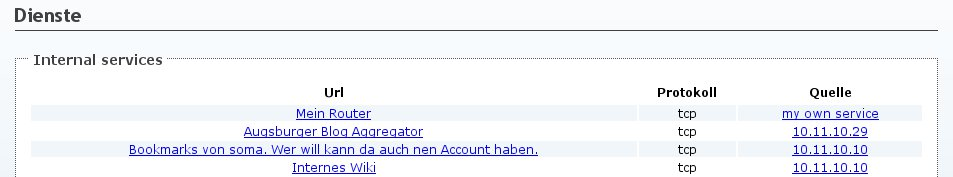
\includegraphics{nameservice-services-table.jpg}


\chapter{Hilf mit bei der Dokumentation}
\label{help-with-documentation:sphinx}\label{help-with-documentation::doc}\label{help-with-documentation:hilf-mit-bei-der-dokumentation}
Eine Dokumentation zu schreiben ist jede Menge Arbeit. Hilfe dabei ist daher
gerne gesehen.


\section{Allgemeine Regeln zur Dokumentation}
\label{help-with-documentation:allgemeine-regeln-zur-dokumentation}\begin{itemize}
\item {} 
Texte sinnvoll durch Überschriften gliedern

\item {} 
Bilder: Nur JPG oder PNG verwenden

\item {} 
Wo möglich verweise auf andere Stellen in der Dokumentation

\item {} 
Erkläre möglichst gut und dabei so kurz wie möglich

\end{itemize}

Zur Erstellung der Dokumentation wird \href{http://sphinx-doc.org}{Sphinx} genutzt.


\section{Installation von Sphinx}
\label{help-with-documentation:installation-von-sphinx}
Viele Linux Distributionen bieten Sphinx als Paket an, unter Debian kann es
installiert werden mit:

\begin{Verbatim}[commandchars=\\\{\}]
aptitude install python\PYGZhy{}sphinx python\PYGZhy{}pygments
\end{Verbatim}

Desweiteren benötigt diese Dokumentation ein angepasstes Theme, das mit
folgendem Befehl installiert werden kann:

\begin{Verbatim}[commandchars=\\\{\}]
easy\PYGZus{}install sphinxjp.themes.basicstrap
\end{Verbatim}

oder alternativ mit

\begin{Verbatim}[commandchars=\\\{\}]
pip install sphinxjp.themes.basicstrap
\end{Verbatim}



\renewcommand{\indexname}{Stichwortverzeichnis}
\printindex
\end{document}
